% XCircuit output "red_realim.tex" for LaTeX input from red_realim.eps
\def\putbox#1#2#3#4{\makebox[0in][l]{\makebox[#1][l]{}\raisebox{\baselineskip}[0in][0in]{\raisebox{#2}[0in][0in]{\scalebox{#3}{#4}}}}}
\def\rightbox#1{\makebox[0in][r]{#1}}
\def\centbox#1{\makebox[0in]{#1}}
\def\topbox#1{\raisebox{-0.60\baselineskip}[0in][0in]{#1}}
\def\midbox#1{\raisebox{-0.20\baselineskip}[0in][0in]{#1}}
   \scalebox{1}{
   \normalsize
   \parbox{6.55208in}{
   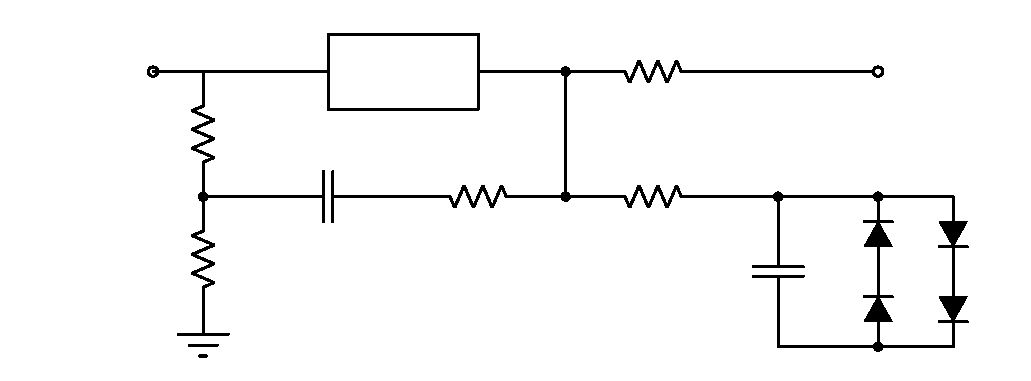
\includegraphics[scale=1]{red_realim}\\
   % translate x=676 y=556 scale 0.38
   \putbox{2.58in}{1.95in}{1.20}{\centbox{\midbox{\textsc{Entrada}}}}%
   \putbox{5.83in}{1.95in}{1.20}{\midbox{$v_{O}$}}%
   \putbox{3.16in}{2.04in}{1.20}{\textbf{-}}%
   \putbox{1.99in}{2.04in}{1.20}{\rightbox{\textbf{+}}}%
   \putbox{0.83in}{1.95in}{1.20}{\rightbox{\midbox{$v_{in}$}}}%
   \putbox{4.83in}{0.62in}{1.20}{\rightbox{\midbox{$C_{18}$}}}%
   \putbox{4.24in}{1.29in}{1.20}{\centbox{$R_{15}$}}%
   \putbox{3.08in}{1.29in}{1.20}{\centbox{$R_{20}$}}%
   \putbox{2.08in}{1.37in}{1.20}{\centbox{$C_8$}}%
   \putbox{4.24in}{2.12in}{1.20}{\centbox{$R_{27}$}}%
   \putbox{1.08in}{1.54in}{1.20}{\rightbox{\midbox{$R_{17}$}}}%
   \putbox{1.08in}{0.70in}{1.20}{\rightbox{\midbox{$R_{18}$}}}%
   } % close 'parbox'
   } % close 'scalebox'
   \vspace{-\baselineskip} % this is not necessary, but looks better
